\documentclass[10pt,twocolumn]{article}

\usepackage[margin=2cm]{geometry}
\usepackage{graphicx}
\usepackage{booktabs}
\usepackage{xcolor}
\usepackage{hyperref}
\usepackage{tikz}
\usepackage{caption}
\usepackage{subcaption}
\usetikzlibrary{positioning,arrows.meta,shapes.geometric,calc,decorations.pathreplacing}

\hypersetup{colorlinks=true,linkcolor=blue!60!black,citecolor=blue!60!black,urlcolor=blue!60!black}

\renewcommand{\abstractname}{\large Abstract}
\newcommand{\keywords}[1]{\par\smallskip\noindent\textbf{Keywords:} #1}

\title{\Large\bfseries How Much Can You Trust This Page?\\[4pt] Consistency-Based Trust Scoring for\\AI-Transcribed Historical Manuscripts}

\author{Derek Lomas\\
\small Source Library / Embassy of the Free Mind\\
\small \texttt{derek@sourcelibrary.org}}

\date{April 2026 --- Preprint}

\begin{document}
\maketitle
\thispagestyle{empty}

\begin{abstract}
\noindent Multimodal large language models can now OCR and translate thousands of historical manuscripts at scale. But how much should a reader trust the result? We introduce a reference-free trust metric based on run-to-run self-consistency: transcribe the same page multiple times and measure agreement using embedding cosine similarity. On a corpus of 50 pages spanning printed books and Leonardo da Vinci's mirror-script notebooks across eight codices, embedding consistency varies from 99\% on printed Latin to 83\% on Leonardo's mirror writing, and all five frontier models tested converge to the same range on handwritten text.

Per-sentence consensus reveals that on printed text, 14/15 sentences are reliably transcribed; on Leonardo's mirror-script, \emph{not a single sentence} is consistent across runs. Comparison against Richter's expert transcriptions shows self-consistency overestimates accuracy by ${\sim}$20 percentage points on manuscript text. Image preprocessing (flipping + contrast) improves consistency from 84\% to 94\%, while reasoning models make performance \emph{worse}---the bottleneck is perceptual, not cognitive. The Leonardo case reveals ``informed confabulation'': topically correct but textually unfaithful output. For historical manuscripts, knowing \emph{what you don't know} is as valuable as the transcription itself.
\end{abstract}

\keywords{OCR, historical manuscripts, self-consistency, trust scoring, Leonardo da Vinci, VLM hallucination, digital humanities}

% ============================================================================
\section{Introduction}

In February 2022, one of the authors encountered a 1497 edition of Ficino's \emph{De Mysteriis} at the Embassy of the Free Mind in Amsterdam. Bound within it was his \emph{Liber de Voluptate}---a Latin dialogue on pleasure that had never been translated into English. This led to Source Library, a project that has since OCR'd and translated over 17,000 historical books (15th--18th c.) using multimodal LLMs.

The pipeline works remarkably well on printed text. But when we turned it to Leonardo da Vinci's mirror-script notebooks, the AI produced fluent Italian about the right topics---but the \emph{specific text changed completely between runs}. Same model, same image, same prompt---different words every time.

\textbf{Contributions:} (1)~Systematic evaluation of LLM OCR consistency across text types, models, and preprocessing. (2)~Evidence that self-consistency overestimates accuracy by ${\sim}$20 points on manuscripts. (3)~A trust taxonomy and consensus tool for digital libraries. (4)~The first assessment of automated transcription on Leonardo's mirror script, revealing ``informed confabulation.''

% --- Figure 1: Core contrast ---
\begin{figure*}[t]
\centering
\begin{subfigure}[t]{0.48\textwidth}
\centering
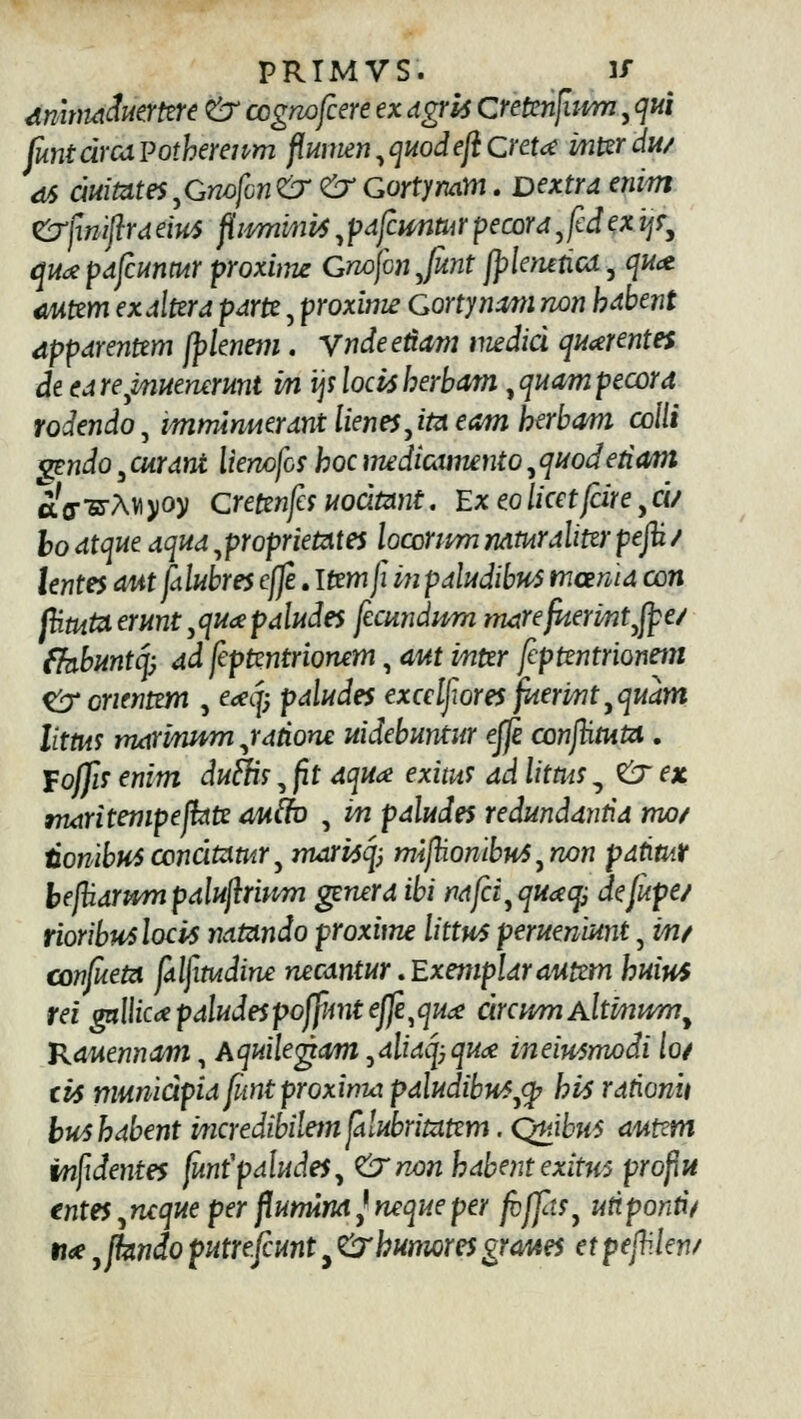
\includegraphics[width=\linewidth]{figures/vitruvius-p33.jpg}
\caption{Vitruvius, \emph{De architectura} (1521). Printed Latin. \textbf{99.1\%} embedding consistency. Five runs produce the same text.}
\end{subfigure}\hfill
\begin{subfigure}[t]{0.48\textwidth}
\centering
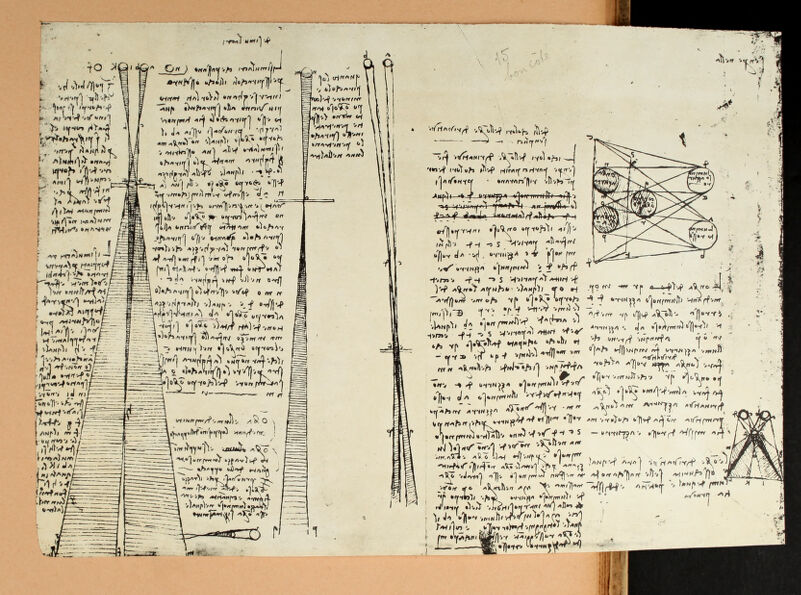
\includegraphics[width=\linewidth]{figures/leonardo-p49.jpg}
\caption{Leonardo, \emph{\'Etudes sur la chevelure} (c.\,1490). Mirror-script. \textbf{82.2\%} embedding consistency. Run lengths: 314--2,939 characters.}
\end{subfigure}
\caption{The core contrast. Printed text is read identically across runs (left). Leonardo's mirror-script produces topically related but textually different output each time (right)---``informed confabulation.''}
\label{fig:contrast}
\end{figure*}

% ============================================================================
\section{Related Work}

\textbf{Historical OCR.} Transkribus achieves CER of 1.7\% on matched training data but degrades to 73\% out-of-domain~\cite{constum2022}. Cl\'erice~\cite{clerice2022} proposed ground-truth-free HTR evaluation. Neudecker et al.~\cite{neudecker2021} noted that ground truth is ``neither feasible nor affordable'' at scale.

\textbf{LLM-based OCR.} Humphries et al.~\cite{humphries2024} showed GPT-4o, Claude, and Gemini achieve CER of 5.7--7\% on 18th--19th c.\ handwriting, outperforming Transkribus by 14\%. Liu et al.~\cite{liu2024} introduced OCRBench, revealing weaknesses in handwritten text.

\textbf{Self-consistency.} Wang et al.~\cite{wang2023} introduced self-consistency decoding (ICLR 2023). Manakul et al.~\cite{manakul2023} formalized this for hallucination detection with SelfCheckGPT (EMNLP 2023). Farquhar et al.~\cite{farquhar2024} introduced semantic entropy (Nature 2024). We adapt these to OCR, where the output is a deterministic function of a fixed image---making disagreement a particularly clean signal.

\textbf{VLM hallucination.} Zhou et al.~\cite{zhou2025} identified ``semantic hallucination'' in scene text. Wang et al.~\cite{wang2025} benchmarked OCR hallucination under degradation (NeurIPS 2025). No prior work has attempted automated transcription of Leonardo's mirror script.

% ============================================================================
\section{Method}

% --- Figure 2: Method overview ---
\begin{figure}[t]
\centering
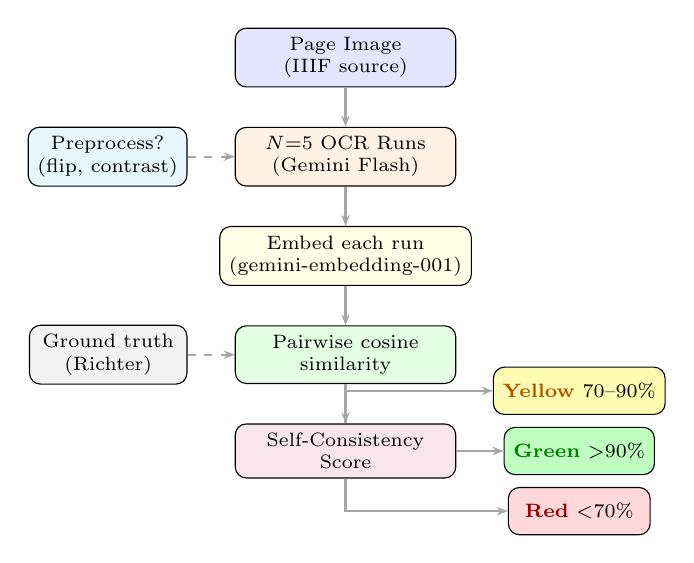
\begin{tikzpicture}[
    node distance=0.5cm,
    box/.style={draw, rounded corners, fill=#1, minimum width=2.8cm, minimum height=0.6cm, font=\scriptsize, align=center},
    arr/.style={-{Stealth[length=4pt]}, thick, gray!70},
]
% Pipeline
\node[box=blue!10] (img) {Page Image\\(IIIF source)};
\node[box=orange!10, below=of img] (ocr) {$N{=}5$ OCR Runs\\(Gemini Flash)};
\node[box=yellow!10, below=of ocr] (embed) {Embed each run\\(gemini-embedding-001)};
\node[box=green!10, below=of embed] (pair) {Pairwise cosine\\similarity};
\node[box=purple!10, below=of pair] (score) {Self-Consistency\\Score};

\draw[arr] (img) -- (ocr);
\draw[arr] (ocr) -- (embed);
\draw[arr] (embed) -- (pair);
\draw[arr] (pair) -- (score);

% Trust output
\node[box=green!25, right=0.6cm of score, minimum width=1.8cm] (green) {\textcolor{green!50!black}{\textbf{Green}} $>$90\%};
\node[box=yellow!30, above=0.15cm of green, minimum width=1.8cm] (yellow) {\textcolor{orange!70!black}{\textbf{Yellow}} 70--90\%};
\node[box=red!15, below=0.15cm of green, minimum width=1.8cm] (red) {\textcolor{red!60!black}{\textbf{Red}} $<$70\%};

\draw[arr] (score) -- (green);
\draw[arr] (score) |- (yellow);
\draw[arr] (score) |- (red);

% Optional: preprocessing
\node[box=cyan!10, left=0.6cm of ocr, minimum width=2cm] (pre) {Preprocess?\\(flip, contrast)};
\draw[arr, dashed] (pre) -- (ocr);

% Optional: ground truth
\node[box=gray!10, left=0.6cm of pair, minimum width=2cm] (gt) {Ground truth\\(Richter)};
\draw[arr, dashed] (gt) -- (pair);
\end{tikzpicture}
\caption{Method overview. Each page is OCR'd $N{=}5$ times, embedded, and scored by pairwise cosine similarity. Optional: image preprocessing before OCR; ground-truth comparison via Richter.}
\label{fig:method}
\end{figure}

\textbf{Corpus.} Source Library contains ${\sim}$17,000 books and 3.35M processed pages. Our evaluation corpus: 50 pages across 13 sources---printed Latin and Italian (Vitruvius, Drebbel, Trattato della pittura, Del moto), a 12th c.\ manuscript (Bodleian Timaeus), and 7 Leonardo mirror-script codices (optics, anatomy, geometry, botany, physiognomy, architecture, flight). Richter's \emph{Literary Works of Leonardo}~\cite{richter1883} provides ground truth.

\textbf{Self-consistency score.} For page image $I$, generate $N$ transcriptions $T_1,\ldots,T_N$ and compute:
$$\textrm{SC}(I) = \frac{1}{\binom{N}{2}} \sum_{i<j} \textrm{sim}(T_i, T_j)$$
We compare: \emph{Jaccard} (word-set overlap), \emph{embedding cosine} (Gemini \texttt{embedding-001}, 768-dim), and \emph{CER}. We use $N{=}5$ and strip metadata tags before comparison.

\textbf{Models.} Gemini 3 Flash, 3.1 Flash Lite, 3 Pro; Claude Sonnet 4, Opus 4.6. Default temperature, no few-shot.

% ============================================================================
\section{Results}

\subsection{Embedding Similarity Is the Right Metric}

\begin{table}[t]
\small
\centering
\caption{Consistency by metric ($N{=}5$, Gemini Flash).}
\label{tab:metrics}
\begin{tabular}{@{}lcccc@{}}
\toprule
Text Type & Jaccard & Embed. & CER & Len.\ Var. \\
\midrule
Printed (p25) & 55\% & \textbf{99.0\%} & 15\% & $\pm$10\% \\
Printed (p33) & 62\% & \textbf{99.1\%} & 5\% & $\pm$2\% \\
Leonardo (p49) & 8\% & \textbf{82.2\%} & 80\% & $\pm$130\% \\
Leonardo (p53) & 6\% & \textbf{84.5\%} & 73\% & $\pm$33\% \\
\bottomrule
\end{tabular}
\end{table}

The embedding--Jaccard \textbf{gap} is diagnostic: 40~pp on printed text (formatting noise) vs.\ 77~pp on Leonardo (confabulation). A large gap signals the model is producing semantically coherent but textually divergent output.

\subsection{All Frontier Models Converge}

Five models on the Bodleian manuscript ($N{=}2$, Jaccard): Gemini Lite 36.7\%*, Opus 27.3\%, Pro 27.0\%, Flash 26.8\%, Sonnet 21.5\%. (*Lite produces pseudo-Latin nonsense.) Models spanning different architectures converge within half a point. The bottleneck is visual perception, not language modeling.

\subsection{Image Preprocessing}

% --- Figure 3: Preprocessing comparison ---
\begin{figure}[t]
\centering
\begin{subfigure}[t]{0.48\columnwidth}
\centering
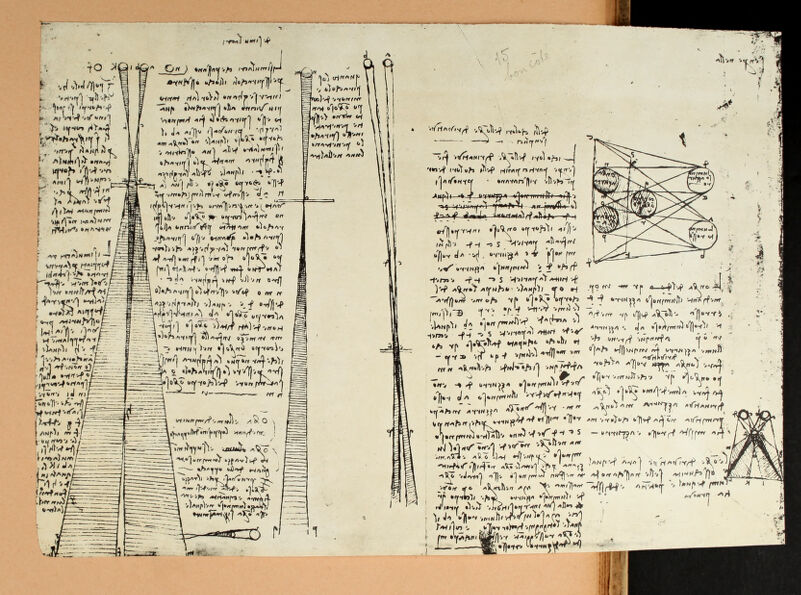
\includegraphics[width=\linewidth]{figures/leonardo-p49.jpg}
\caption{Original mirror-script\\Embedding: 84.0\%}
\end{subfigure}\hfill
\begin{subfigure}[t]{0.48\columnwidth}
\centering
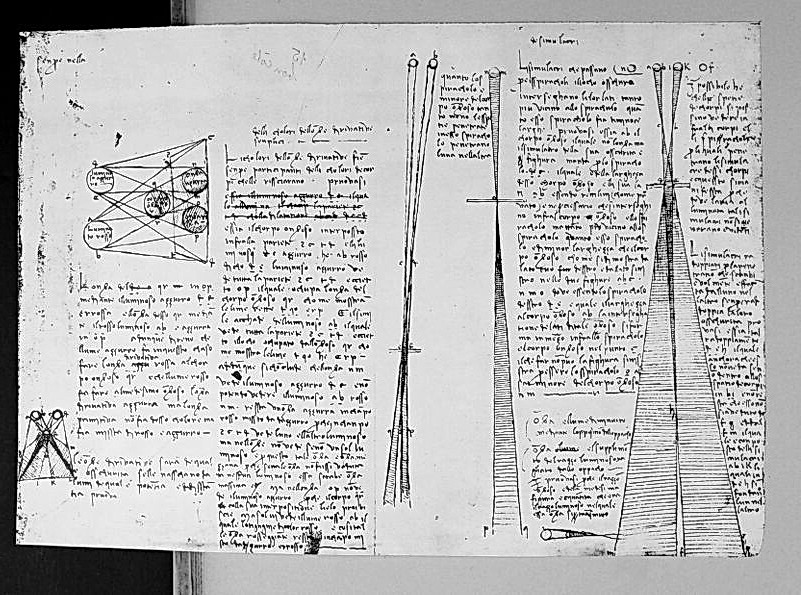
\includegraphics[width=\linewidth]{figures/leonardo-p49-processed.jpg}
\caption{Flipped + contrast\\Embedding: \textbf{94.4\%}}
\end{subfigure}
\caption{Best preprocessing: horizontal flip + grayscale + contrast enhancement. Closes half the gap to printed text (84\%$\to$94\% vs.\ 99\% printed baseline).}
\label{fig:preprocess-images}
\end{figure}

Ten methods tested on Leonardo p49 (Fig.~\ref{fig:preprocess-images},~\ref{fig:preprocess-chart}). \textbf{Flip + contrast} achieves 94.4\%---closing half the gap to printed text. Binarization and denoising \emph{hurt}: the model needs rich grayscale data. On diagram pages, flipping can introduce hallucinated text (98.8\%$\to$88.8\%), motivating selective preprocessing.

\begin{figure}[t]
\centering
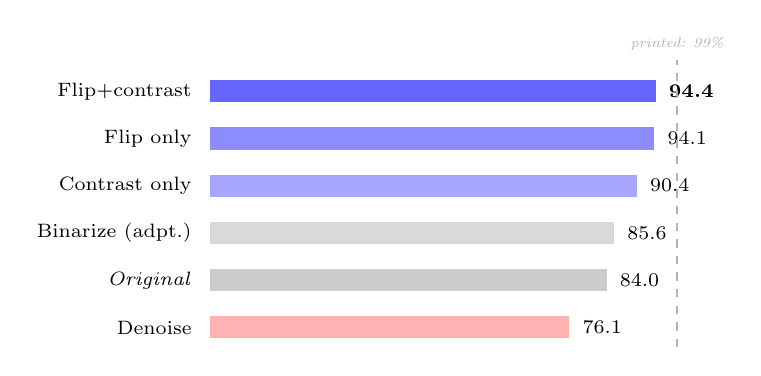
\begin{tikzpicture}[
    bar/.style={fill=#1, minimum height=0.28cm, anchor=west},
    lbl/.style={anchor=east, font=\scriptsize},
]
\def\s{0.06}
\node[lbl] at (-0.1, 3.1) {Flip+contrast};
\node[bar=blue!60, minimum width=94.4*\s cm] at (0, 3.1) {};
\node[font=\scriptsize, anchor=west] at (94.4*\s+0.05, 3.1) {\textbf{94.4}};

\node[lbl] at (-0.1, 2.5) {Flip only};
\node[bar=blue!45, minimum width=94.1*\s cm] at (0, 2.5) {};
\node[font=\scriptsize, anchor=west] at (94.1*\s+0.05, 2.5) {94.1};

\node[lbl] at (-0.1, 1.9) {Contrast only};
\node[bar=blue!35, minimum width=90.4*\s cm] at (0, 1.9) {};
\node[font=\scriptsize, anchor=west] at (90.4*\s+0.05, 1.9) {90.4};

\node[lbl] at (-0.1, 1.3) {Binarize (adpt.)};
\node[bar=gray!30, minimum width=85.6*\s cm] at (0, 1.3) {};
\node[font=\scriptsize, anchor=west] at (85.6*\s+0.05, 1.3) {85.6};

\node[lbl] at (-0.1, 0.7) {\textit{Original}};
\node[bar=gray!40, minimum width=84.0*\s cm] at (0, 0.7) {};
\node[font=\scriptsize, anchor=west] at (84.0*\s+0.05, 0.7) {84.0};

\node[lbl] at (-0.1, 0.1) {Denoise};
\node[bar=red!30, minimum width=76.1*\s cm] at (0, 0.1) {};
\node[font=\scriptsize, anchor=west] at (76.1*\s+0.05, 0.1) {76.1};

\draw[dashed, gray!60] (99*\s, -0.15) -- (99*\s, 3.5) node[above, font=\tiny\itshape] {printed: 99\%};
\end{tikzpicture}
\caption{Embedding consistency (\%) by preprocessing method on Leonardo p49. Dashed line = printed text baseline.}
\label{fig:preprocess-chart}
\end{figure}

\subsection{Reasoning Makes It Worse}

Gemini Pro with extended thinking (4,096--8,192 tokens): embedding drops from Flash's 86\% to 64--81\%, with frequent zero-character outputs. The model over-constrains itself, recognizing it cannot decode individual reversed letterforms. The bottleneck is \textbf{perceptual, not cognitive}.

\subsection{Consistency Tracks Text Density, Not Topic}

% --- Figure 4: Consistency bands ---
\begin{figure}[t]
\centering
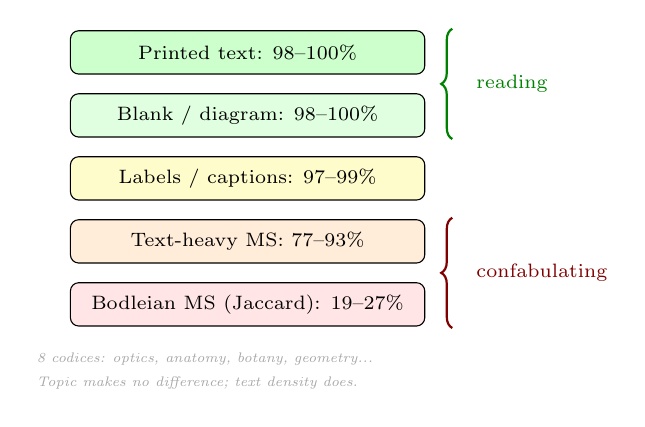
\begin{tikzpicture}[
    band/.style={draw, rounded corners=3pt, minimum width=4.5cm, minimum height=0.55cm, font=\scriptsize, align=center},
    note/.style={font=\tiny\itshape, gray!70},
]
\node[band, fill=green!20] (p) at (0, 2.4) {Printed text: 98--100\%};
\node[band, fill=green!12] (b) at (0, 1.6) {Blank / diagram: 98--100\%};
\node[band, fill=yellow!20] (l) at (0, 0.8) {Labels / captions: 97--99\%};
\node[band, fill=orange!15] (t) at (0, 0.0) {Text-heavy MS: 77--93\%};
\node[band, fill=red!10] (m) at (0, -0.8) {Bodleian MS (Jaccard): 19--27\%};

\draw[decorate, decoration={brace, amplitude=4pt, mirror}, thick, green!50!black]
    (2.6, 2.7) -- (2.6, 1.3) node[midway, right=5pt, font=\scriptsize] {reading};
\draw[decorate, decoration={brace, amplitude=4pt, mirror}, thick, red!50!black]
    (2.6, 0.3) -- (2.6, -1.1) node[midway, right=5pt, font=\scriptsize] {confabulating};

\node[note, anchor=west] at (-2.8, -1.5) {8 codices: optics, anatomy, botany, geometry...};
\node[note, anchor=west] at (-2.8, -1.8) {Topic makes no difference; text density does.};
\end{tikzpicture}
\caption{Embedding consistency bands by page content type across 8 Leonardo codices. Subject matter is irrelevant; visual complexity determines consistency.}
\label{fig:bands}
\end{figure}

Across 8 codices (optics, anatomy, water, flight, geometry, botany, physiognomy, architecture), pages cluster by content type (Fig.~\ref{fig:bands}): blank/diagram (100\%), labels (97--99\%), text-heavy MS (77--93\%), printed (99\%+). An accidental control: \emph{Del moto e misura dell'acqua} (99.7\%) turns out to be a printed compilation---indistinguishable from other printed books.

\subsection{Sentence-Level: Zero Green on Leonardo}

% --- Figure 5: Sentence-level comparison ---
\begin{figure}[t]
\centering
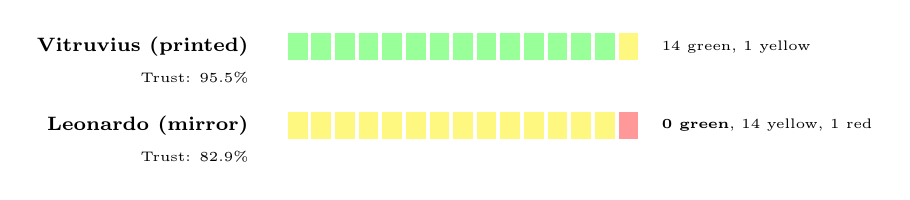
\begin{tikzpicture}[
    cell/.style={minimum width=0.25cm, minimum height=0.35cm},
]
% Vitruvius
\node[font=\scriptsize\bfseries, anchor=east] at (-0.2, 1.0) {Vitruvius (printed)};
\node[font=\tiny, anchor=east] at (-0.2, 0.6) {Trust: 95.5\%};
\foreach \i in {1,...,14} {
    \node[cell, fill=green!40] at (\i*0.3, 1.0) {};
}
\node[cell, fill=yellow!50] at (15*0.3, 1.0) {};
\node[font=\tiny, anchor=west] at (15*0.3+0.3, 1.0) {14 green, 1 yellow};

% Leonardo
\node[font=\scriptsize\bfseries, anchor=east] at (-0.2, -0.0) {Leonardo (mirror)};
\node[font=\tiny, anchor=east] at (-0.2, -0.4) {Trust: 82.9\%};
\foreach \i in {1,...,14} {
    \node[cell, fill=yellow!50] at (\i*0.3, 0.0) {};
}
\node[cell, fill=red!40] at (15*0.3, 0.0) {};
\node[font=\tiny, anchor=west] at (15*0.3+0.3, 0.0) {\textbf{0 green}, 14 yellow, 1 red};
\end{tikzpicture}
\caption{Per-sentence trust ($N{=}5$). Each cell = one sentence. On Leonardo, \textbf{not a single sentence} is reliably reproduced across runs. The page-level score (82.9\%) hides this.}
\label{fig:sentences}
\end{figure}

Per-sentence consensus ($N{=}5$): Vitruvius (printed) scores 95.5\% trust with 14/15 green sentences. Leonardo scores 82.9\% trust with \textbf{0/15 green}---every sentence is yellow or red (Fig.~\ref{fig:sentences}). The page-level score misleadingly suggests acceptable quality.

\subsection{The Calibration Gap}

% --- Figure 6: Calibration gap ---
\begin{figure}[t]
\centering
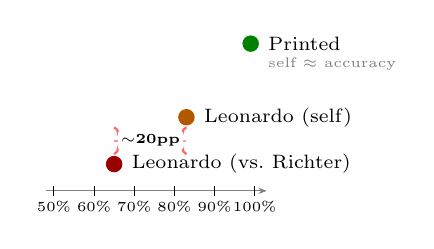
\begin{tikzpicture}[scale=0.85]
\def\s{0.06}
% Axis
\draw[-{Stealth[length=3pt]}, gray] (48*\s,0) -- (103*\s,0);
\foreach \x in {50,60,70,80,90,100}
    \draw (\x*\s, -0.08) -- (\x*\s, 0.08) node[below=2pt, font=\tiny] {\x\%};

% Printed
\fill[green!50!black] (99*\s, 2.2) circle (3.5pt);
\node[font=\scriptsize, anchor=west] at (99*\s+0.12, 2.2) {Printed};
\node[font=\tiny, gray, anchor=west] at (99*\s+0.12, 1.9) {self $\approx$ accuracy};

% Leonardo self
\fill[orange!70!black] (83*\s, 1.1) circle (3.5pt);
\node[font=\scriptsize, anchor=west] at (83*\s+0.12, 1.1) {Leonardo (self)};

% Leonardo accuracy
\fill[red!60!black] (65*\s, 0.4) circle (3.5pt);
\node[font=\scriptsize, anchor=west] at (65*\s+0.12, 0.4) {Leonardo (vs.\ Richter)};

% Gap bracket
\draw[decorate, decoration={brace, amplitude=3pt}, thick, red!60]
    (83*\s, 0.55) -- (83*\s, 0.95);
\draw[decorate, decoration={brace, amplitude=3pt, mirror}, thick, red!60]
    (65*\s, 0.55) -- (65*\s, 0.95);
\draw[thick, red!40] (65*\s, 0.75) -- (83*\s, 0.75);
\node[font=\tiny\bfseries, fill=white, inner sep=1pt] at (74*\s, 0.75) {${\sim}$20pp};
\end{tikzpicture}
\caption{The calibration gap. Self-consistency (83\%) overestimates accuracy (65\%) by ${\sim}$20 points on Leonardo manuscripts. No gap on printed text.}
\label{fig:gap}
\end{figure}

Against Richter's expert transcriptions~\cite{richter1883}: self-consistency is 83--88\%, but accuracy is only 65--67\%---a \textbf{${\sim}$20-point overestimate} (Fig.~\ref{fig:gap}). The model agrees with itself more than with the expert, because it consistently generates plausible text about the right topic.

\subsection{Printed Leonardo Control}

\begin{figure}[t]
\centering
\begin{subfigure}[t]{0.48\columnwidth}
\centering
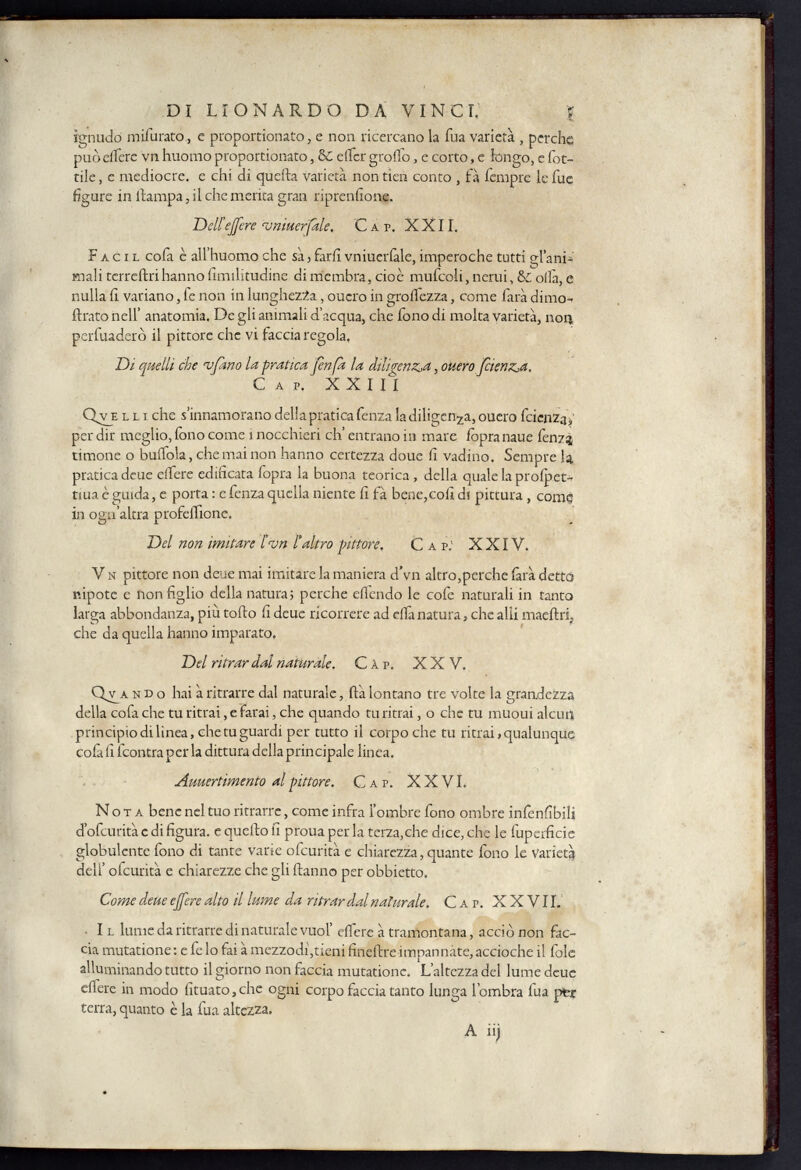
\includegraphics[width=\linewidth]{figures/trattato-p30.jpg}
\caption{Printed \emph{Trattato} (1651)\\Embedding: \textbf{99.6\%}}
\end{subfigure}\hfill
\begin{subfigure}[t]{0.48\columnwidth}
\centering
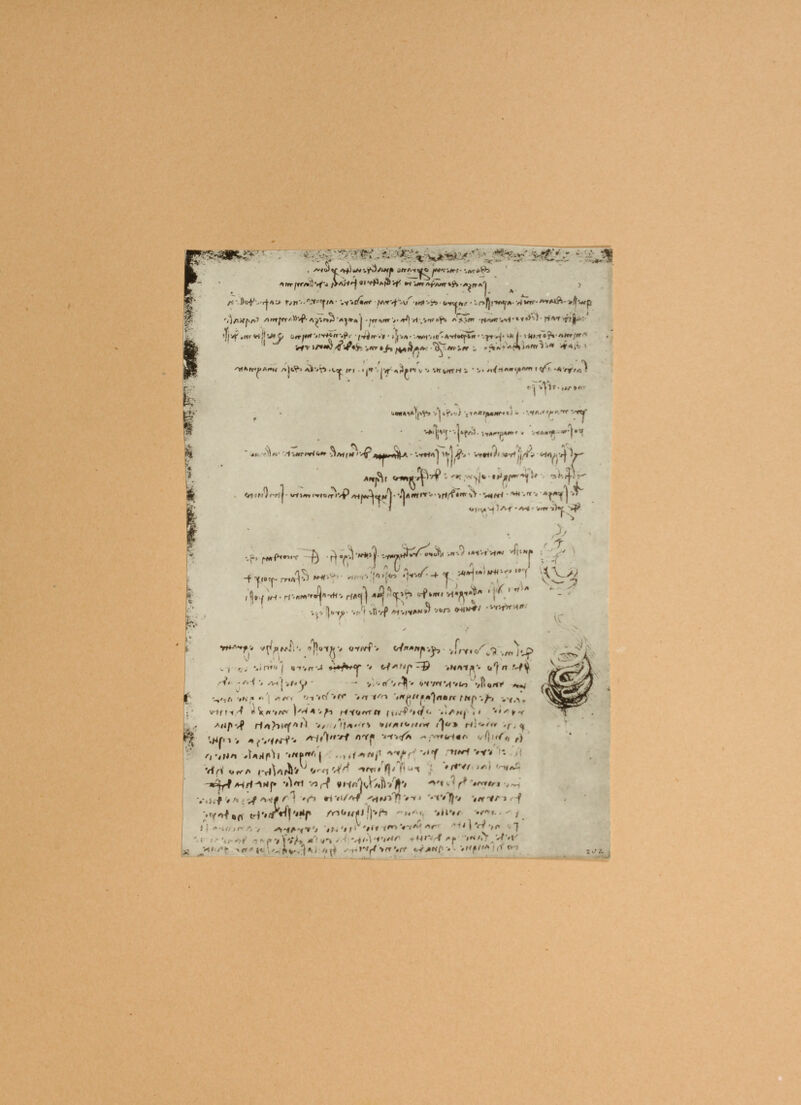
\includegraphics[width=\linewidth]{figures/anatomy-p25.jpg}
\caption{MS Anatomy (Windsor)\\Embedding: \textbf{77.8\%}}
\end{subfigure}
\caption{Same author, different media. The model reads printed Leonardo at 99.6\% but scores only 77.8\% on his manuscripts. The failure is purely handwriting perception.}
\label{fig:printed-vs-ms}
\end{figure}

The \emph{Trattato della pittura} (1651)---Leonardo's text in printed form---scores 98--99.6\% (Fig.~\ref{fig:printed-vs-ms}a). The model reads printed Leonardo perfectly. The failure is purely handwriting perception.

% ============================================================================
\section{Discussion}

\textbf{Informed confabulation} is not random hallucination---the model demonstrates genuine understanding of what Leonardo writes \emph{about}. But it samples text from a learned distribution of ``plausible Italian about [topic]'' rather than decoding the image. The embedding--Jaccard gap (77~pp) quantifies this; run length variation ($\pm$130\%) confirms it.

\textbf{Consensus as enhancement.} Multi-run data can build confidence-annotated transcriptions: keep consistent fragments, mark uncertain ones. This transforms consistency from a passive label into an active tool---preserving what the model \emph{can} read while honestly marking what it cannot.

\textbf{For digital libraries} processing at scale: printed books ($>$95\% of most collections) are production-quality. The ${\sim}$5\% of manuscripts need trust indicators. Self-consistency scoring automates triage at negligible cost versus expert review.

\textbf{Limitations.} Small corpus (50 pages). Richter comparison limited to 2 pages. Gemini embeddings evaluate Gemini OCR (potential bias). Training data contamination and temperature dependence remain unexplored.

% ============================================================================
\section{Conclusion}

Self-consistency via embedding similarity provides a practical, reference-free quality signal for AI-transcribed historical documents---but one that overestimates accuracy by ${\sim}$20 points on difficult manuscripts. Key findings: all frontier models converge on manuscripts; image preprocessing outperforms reasoning; consistency tracks text density, not topic; and on Leonardo's mirror-script, not a single sentence is reliably transcribed. For Leonardo's notebooks, the AI knows what he writes about, but cannot yet read what he wrote.

% ============================================================================
{\small
\bibliographystyle{plain}
\begin{thebibliography}{11}
\bibitem{constum2022} T.~Constum et al. Impact of training set size on HTR for medieval Latin manuscripts. \emph{DAS}, 2022.
\bibitem{clerice2022} T.~Cl\'erice. Evaluating deep learning for word segmentation of scripta continua. \emph{JOCCH}, 15(3), 2022.
\bibitem{neudecker2021} C.~Neudecker et al. A survey of OCR evaluation tools and metrics. \emph{HIP}, 2021.
\bibitem{humphries2024} D.~Humphries et al. Unlocking the archives: Using LLMs to transcribe handwritten historical documents. \emph{arXiv:2407.12437}, 2024.
\bibitem{liu2024} Y.~Liu et al. OCRBench: On the hidden mystery of OCR in large multimodal models. \emph{arXiv:2305.07895}, 2024.
\bibitem{wang2023} X.~Wang et al. Self-consistency improves chain of thought reasoning in language models. \emph{ICLR}, 2023.
\bibitem{manakul2023} P.~Manakul et al. SelfCheckGPT: Zero-resource hallucination detection. \emph{EMNLP}, 2023.
\bibitem{farquhar2024} S.~Farquhar et al. Detecting hallucinations in LLMs using semantic entropy. \emph{Nature}, 630:625--630, 2024.
\bibitem{zhou2025} Y.~Zhou et al. Semantic hallucination in scene text recognition. 2025.
\bibitem{wang2025} Z.~Wang et al. Seeing is believing? OCR hallucination under visual degradation. \emph{NeurIPS}, 2025.
\bibitem{richter1883} J.~P.~Richter. \emph{The Literary Works of Leonardo da Vinci}. Sampson Low, 1883.
\end{thebibliography}
}

\end{document}
